% Copyright 2005 by Till Tantau <tantau@cs.tu-berlin.de>.
%
% This program can be redistributed and/or modified under the terms
% of the LaTeX Project Public License Distributed from CTAN
% archives in directory macros/latex/base/lppl.txt.


\section{Nodes}

\label{section-nodes}

\subsection{Nodes and Their Shapes}

\tikzname\ offers an easy way of adding so-called \emph{nodes} to your
pictures. In the simplest case, a node is just some text that is
placed at some coordinate. However, a node can also have a border
drawn around it or have a more complex background and
foreground. Indeed, some nodes do not have a text at all, but consist
solely of the background. You can name nodes so that you can reference
their coordinates later in the picture. However, \emph{nodes cannot be
  referenced across different pictures}. 

There are no special \TeX\ commands for adding a node to a picture; rather,
there is path operation called |node| for this. Nodes are created
whenever \tikzname\ encounters |node| or |coordinate| at a point on a
path where it would expect a normal path operation (like |-- (1,1)| or
|sin (1,1)|). It is also possible to give node specifications
\emph{inside} certain path operations as explained later.

The node operation is typically followed by some options, which apply
only to the node. Then, you can optionally \emph{name} the node by
providing a name in round braces. Lastly, for the |node| operation you
must provide some label text for the node in curly braces, while for
the |coordinate| operation you may not. The node is placed at the
current position of the path \emph{after the path has been
  drawn}. Thus, all nodes are drawn ``on top'' of the path and
retained until the path is complete. If there are several nodes on a
path, they are drawn on top of the path in the order they are
encountered. 

\begin{codeexample}[]
\tikz \fill[fill=examplefill]
     (0,0) node {first node}
  -- (1,1) node {second node}
  -- (0,2) node {third node};
\end{codeexample}

The syntax for specifying nodes is the following:
\begin{pathoperation}{node}{\opt{|[|\meta{options}|]|}\opt{|(|\meta{name}|)|}%
    \opt{|at(|\meta{coordinate}|)|}\opt{\marg{text}}}
  The effect of |at| is to place the node at the coordinate given
  after |at| and not, as would normally be the case, at the last
  position. The |at| syntax is not available when a node is given
  inside a path operation (it would not make any sense, there).
  
  The |(|\meta{name}|)| is a name for later reference and it is
  optional. You may also add the option |name=|\meta{name} to the
  \meta{option} list; it has the same effect.

  \begin{itemize}
    \itemoption{name}|=|\meta{node name}
    assigns a name to the node for later reference. Since this is a
    ``high-level'' name (drivers never know of it), you can use spaces,
    number, letters, or whatever you like when naming a node. Thus, you
    can name a node just |1| or perhaps |start of chart| or even
    |y_1|. Your node name should \emph{not} contain any punctuation like
    a dot, a comma, or a colon since these are used to detect what kind
    of coordinate you mean when you reference a node. 
  \end{itemize}

  The \meta{options} is an optional list of options that \emph{apply
    only to the node} and have no effect outside. The other way round,
  most ``outside'' options also apply to the node, but not all. For
  example, the ``outside'' rotation does not apply to nodes (unless some
  special options are used, sigh). Also, the outside path action, like
  |draw| or |fill|, never applies to the node and must be given in the
  node (unless some special other options are used, deep sigh).

  As mentioned before, we can add a border and even a background to a
  node:  
\begin{codeexample}[]
\tikz \fill[fill=examplefill]
      (0,0) node {first node}
   -- (1,1) node[draw] {second node}
   -- (0,2) node[fill=red!20,draw,double,rounded corners] {third node};
\end{codeexample}

  The ``border'' is actually just a special case of a much more general
  mechanism. Each node has a certain \emph{shape} which, by default, is
  a rectangle. However, we can also ask \tikzname\ to use a circle shape
  instead or an ellipse shape (you have to include |pgflibraryshapes| for
  the latter shape): 

\begin{codeexample}[]
\tikz \fill[fill=examplefill]
      (0,0) node{first node}
   -- (1,1) node[ellipse,draw] {second node}
   -- (0,2) node[circle,fill=red!20] {third node};
\end{codeexample}

  In the future, there might be much more complicated shapes available
  such as, say, a shape for a resistor or a shape for a state of a
  finite automaton or a shape for a \textsc{uml} class. Unfortunately,
  creating new shapes is a bit tricky and makes it necessary to use the
  basic layer directly. Life is hard.

  To select the shape of a node, the following option is used:
  \begin{itemize}
    \itemoption{shape}|=|\meta{shape name}
    select the shape either of the current node or, when this option is
    not given inside a node but somewhere outside, the shape of all
    nodes in the current scope.%
    \indexoption{\meta{shape name}}

    Since this option is used often, you can leave out the
    |shape=|. When \tikzname\ encounters an option like |circle|
    that it does not know, it will, after everything else has failed,
    check whether this option is the name of some shape. If so, that
    shape is selected as if you had said |shape=|\meta{shape name}.

    By default, the following shapes are available: |rectangle|,
    |circle|, |coordinate|, and, when the package |pgflibraryshapes| is
    loaded, also |ellipse|. Details of these shapes, like their anchors
    and size options, are discussed in Section~\ref{section-the-shapes}.
  \end{itemize}
  
  The following styles influences how nodes are rendered:
  \begin{itemize}
    \itemstyle{every node}
    This style is installed at the beginning of every node. 
\begin{codeexample}[]
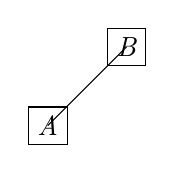
\begin{tikzpicture}
  \tikzstyle{every node}=[draw] 
  \draw (0,0) node {A} -- (1,1) node {B};
\end{tikzpicture}
\end{codeexample}

    \itemstyle{every \meta{shape} node}
    These styles are installed at the beginning of a node of a given
    \meta{shape}. For example, |every rectangle node| is used for
    rectangle nodes, and so on.
\begin{codeexample}[]
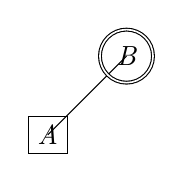
\begin{tikzpicture}
  \tikzstyle{every rectangle node}=[draw] 
  \tikzstyle{every circle node}=   [draw,double] 
  \draw (0,0) node[rectangle] {A} -- (1,1) node[circle] {B};
\end{tikzpicture}
\end{codeexample}
  \end{itemize}
\end{pathoperation}

The is a special syntax for specifying ``light-weighed'' nodes:

\begin{pathoperation}{coordinate}{\opt{|[|\meta{options}|]|}|(|\meta{name}|)|\opt{|at(|\meta{coordinate}|)|}}
  This has the same effect as

  |node[shape=coordinate][|\meta{options}|](|\meta{name}|)at(|\meta{coordinate}|){}|,
  
  where the |at| part might be missing.
\end{pathoperation}



\subsection{Multi-Part Nodes}

Most nodes just have a single simple text label. However, nodes of a
more complicated shapes might be made up from several \emph{node
  parts}. For example, in automata theory a so-called Moore state has
a state name, drawn in the upper part of the state circle, and an
output text, drawn in the lower part of the state circle. These two
parts are quite independent. Similarly, a \textsc{uml} class shape
would have a name part, a method part, and an attributes
part. Different molecule shape might use parts for the different atoms
to be drawn at the different positions, and so on.

Both \pgfname\ and \tikzname\ support such multipart nodes. On the
lower level, \pgfname\ provides a system for specifying that a shape
consists of several parts. On the \tikzname\ level, you specify the
different node parts by using the following command:

\begin{command}{\nodepart\marg{part name}}
  This command can only be used inside the \meta{text} argument of a
  |node| path operation. It works a little bit like a |\part| command
  in \LaTeX. It will stop the typesetting of whatever node part was
  typeset until now and then start putting all following text into the
  node part named \meta{part name}---until another |\partname| is
  encountered or until the node \meta{text} ends.

\begin{codeexample}[]
\begin{tikzpicture}
  \node [state with output,draw,double,fill=red!20]
  {
    % No \nodepart has been used, yet. So, the following is put in the
    % ``text'' node part by default.
    $q_1$ 
    \nodepart{output} % Ok, end ``text'' part, start ``output'' part
    $00$
  }; % output part ended.
\end{tikzpicture}
\end{codeexample}

  You will have to lookup which parts are defined by a shape.

  The following styles influences node parts:
  \begin{itemize}
    \itemstyle{every \meta{part name} node part}
    This style is installed at the beginning of every node part named
    \meta{part name}. 
\begin{codeexample}[]
\tikzstyle{every output node part}=[red] 
\tikz \node [state with output,draw] {$q_1$ \nodepart{output} $00$};
\end{codeexample}
  \end{itemize}
\end{command}



\subsection{Options for the Text in  Nodes}

The simplest option for the text in nodes is its color. Normally, this
color is just the last color installed using |color=|, possibly
inherited from another scope. However, it is possible to specificly
set the color used for text using the following option:

\begin{itemize}
  \itemoption{text}|=|\meta{color}
  Sets the color to be used for text labels. A |color=| option
  will immediately override this option.
\begin{codeexample}[]
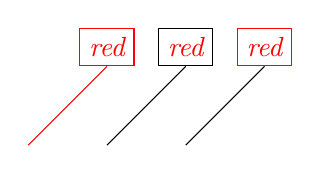
\begin{tikzpicture}
  \draw[red]       (0,0) -- +(1,1) node[above]     {red};
  \draw[text=red]  (1,0) -- +(1,1) node[above]     {red};
  \draw            (2,0) -- +(1,1) node[above,red] {red};
\end{tikzpicture}
\end{codeexample}
\end{itemize}

Next, you may wish to adjust the font used for the text. Use the
following option for this:
\begin{itemize}
  \itemoption{font}|=|\meta{font commands}
  Sets the font used for text labels. 
\begin{codeexample}[]
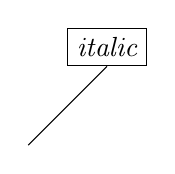
\begin{tikzpicture}
  \draw[font=\itshape] (1,0) -- +(1,1) node[above] {italic};
\end{tikzpicture}
\end{codeexample}
  A perhaps more useful example is the following:

\begin{codeexample}[]
\tikzstyle{every text node part}=[font=\itshape] 
\tikzstyle{every output node part}=[font=\footnotesize]
\tikzstyle{every state with output node}=[draw]
\tikz \node [state with output] {state \nodepart{output} output};
\end{codeexample}
\end{itemize}


Normally, when a node is typeset, all the text you give in the braces
is but in one long line (in an |\hbox|, to be precise) and the node
will become as wide as necessary.

You can change this behaviour using the following options. They allow
you to limit the width of a node (naturally, at the expense of its
height).

\begin{itemize}
  \itemoption{text width}|=|\meta{dimension}
  This option will put the text of a node in a box of the given width
  (more precisely, in a |{minipage}| of this width; for plain \TeX\ a
  rudimentary ``minipage emulation'' is used).

  If the node text is not as wide as \meta{dimension}, it will
  nevertheless be put in a box of this width. If it is larger, line
  breaking will be done.

  By default, when this option is given, a ragged right border will be
  used. This is sensible since, typically, these boxes are narrow and
  justifying the text looks ugly.
\begin{codeexample}[]
\tikz \draw (0,0) node[fill=examplefill,text width=3cm]
  {This is a demonstration text for showing how line breaking works.};  
\end{codeexample}
  \itemoption{text justified}
  causes the text to be justified instead of (right)ragged. Use this
  only with pretty broad nodes.
{%
\hbadness=10000
\begin{codeexample}[]
\tikz \draw (0,0) node[fill=examplefill,text width=3cm,text justified]
  {This is a demonstration text for showing how line breaking works.};  
\end{codeexample}
}
  In the above example, \TeX\ complains (rightfully) about three very
  badly typeset lines. (For this manual I asked \TeX\ to stop
  complaining by using |\hbadness=10000|, but this is a foul deed,
  indeed.) 
  \itemoption{text ragged}
  causes the text to be typeset with a ragged right. This uses the
  original plain \TeX\ definition of a ragged right border, in which
  \TeX\ will try to balance the right border as well as possible. This
  is the default.
\begin{codeexample}[]
\tikz \draw (0,0) node[fill=examplefill,text width=3cm,text ragged]
  {This is a demonstration text for showing how line breaking works.};  
\end{codeexample}
  \itemoption{text badly ragged}
  causes the right border to be ragged in the \LaTeX-style, in which
  no balancing occurs. This looks ugly, but it may be useful for very
  narrow boxes and when you wish to avoid hyphenations.
\begin{codeexample}[]
\tikz \draw (0,0) node[fill=examplefill,text width=3cm,text badly ragged]
  {This is a demonstration text for showing how line breaking works.};  
\end{codeexample}
  \itemoption{text centered}
  centers the text, but tries to balance the lines.
\begin{codeexample}[]
\tikz \draw (0,0) node[fill=examplefill,text width=3cm,text centered]
  {This is a demonstration text for showing how line breaking works.};  
\end{codeexample}
  \itemoption{text badly centered}
  centers the text, without balancing the lines.
\begin{codeexample}[]
\tikz \draw (0,0) node[fill=examplefill,text width=3cm,text badly centered]
  {This is a demonstration text for showing how line breaking works.};  
\end{codeexample}
\end{itemize}



\subsection{Placing Nodes Using Anchors}

When you place a node at some coordinate, the node is centered on this
coordinate by default. This is often undesirable and it would be
better to have the node to the right or above the actual coordinate.

\pgfname\ uses a so-called anchoring mechanism to give you a very fine
control over the placement. The idea is simple: Imaging a node of
rectangular shape of a certain size. \pgfname\ defines numerous anchor
positions in the shape. For example to upper right corner is called,
well, not ``upper right anchor,'' but the |north east| anchor of the
shape. The center of the shape has an anchor called |center| on top of
it, and so on. Here are some examples (a complete list is given in
Section~\ref{section-the-shapes}).

\medskip\noindent
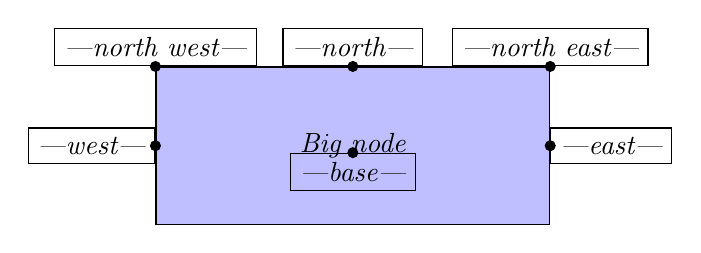
\begin{tikzpicture}
  \path node[minimum height=2cm,minimum width=5cm,fill=blue!25](x) {Big node};
  \fill (x.north)      circle (2pt) node[above] {|north|}
        (x.north east) circle (2pt) node[above] {|north east|}
        (x.north west) circle (2pt) node[above] {|north west|}
        (x.west) circle (2pt)       node[left]  {|west|}
        (x.east) circle (2pt)       node[right] {|east|}
        (x.base) circle (2pt)       node[below] {|base|};
\end{tikzpicture}

Now, when you place a node at a certain coordinate, you can ask \tikzname\
to place the node shifted around in such a way that a certain
anchor is at the coordinate. In the following example, we ask \tikzname\
to shift the first node such that its  |north east| anchor is at
coordinate |(0,0)| and that the |west| anchor of the second node is at
coordinate |(1,1)|.

\begin{codeexample}[]
\tikz \draw           (0,0) node[anchor=north east] {first node}
            rectangle (1,1) node[anchor=west] {second node};
\end{codeexample}

Since the default anchor is |center|, the default behaviour is to
shift the node in such a way that it is centered on the current
position.

\begin{itemize}
  \itemoption{anchor}|=|\meta{anchor name}
  causes the node to be shifted such that it's anchor \meta{anchor
  name} lies on the current coordinate.

  The only anchor that is present in all shapes is |center|. However,
  most shapes will at least define anchors in all ``compass
  directions.'' Furthermore, the standard shapes also define a |base|
  anchor, as well as |base west| and |base east|, for placing things on
  the baseline of the text.
  
  The standard shapes also define a |mid| anchor (and |mid west| and
  |mid east|). This anchor is half the height of the character ``x''
  above the base line. This anchor is useful for vertically centering
  multiple nodes that have different heights and depth. Here is an
  example:
\begin{codeexample}[]
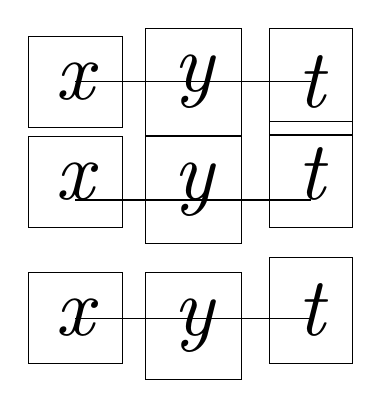
\begin{tikzpicture}[scale=3,transform shape]
  % First, center alignment -> wobbles
  \draw[anchor=center] (0,1)  node{x} -- (0.5,1)  node{y} -- (1,1)  node{t};
  % Second, base alignment -> no wobble, but too high
  \draw[anchor=base]   (0,.5) node{x} -- (0.5,.5) node{y} -- (1,.5) node{t};
  % Third, mid alignment
  \draw[anchor=mid]    (0,0)  node{x} -- (0.5,0)  node{y} -- (1,0)  node{t};
\end{tikzpicture}
\end{codeexample}
\end{itemize}

Unfortunately, while perfectly logical, it is often rather
counter-intuitive that in order to place a node \emph{above} a given
point, you need to specify the |south| anchor. For this reason, there
are some useful options that allow you to select the standard anchors
more intuitively:
\begin{itemize}
  \itemoption{above}\opt{|=|\meta{offset}}
  does the same as |anchor=south|. If the \meta{offset} is specified,
  the node is additionally shifted upwards by the given
  \meta{offset}. 
\begin{codeexample}[]
\tikz \fill (0,0) circle (2pt) node[above] {above};
\end{codeexample}
\begin{codeexample}[]
\tikz \fill (0,0) circle (2pt) node[above=2pt] {above};
\end{codeexample}
  \itemoption{above left}\opt{|=|\meta{offset}}
  does the same as |anchor=south east|. If the \meta{offset} is
  specified, the node is additionally shifted upwards and right by
  \meta{offset}. 
\begin{codeexample}[]
\tikz \fill (0,0) circle (2pt) node[above left] {above left};
\end{codeexample}
\begin{codeexample}[]
\tikz \fill (0,0) circle (2pt) node[above left=2pt] {above left};
\end{codeexample}
  \itemoption{above right}\opt{|=|\meta{offset}}
  does the same as |anchor=south west|.
\begin{codeexample}[]
\tikz \fill (0,0) circle (2pt) node[above right] {above right};
\end{codeexample}
  \itemoption{left}\opt{|=|\meta{offset}}
  does the same as |anchor=east|.
\begin{codeexample}[]
\tikz \fill (0,0) circle (2pt) node[left] {left};
\end{codeexample}
  \itemoption{right}\opt{|=|\meta{offset}}
  does the same as |anchor=west|.
  \itemoption{below}\opt{|=|\meta{offset}}
  does the same as |anchor=north|.
  \itemoption{below left}\opt{|=|\meta{offset}}
  does the same as |anchor=north east|.
  \itemoption{below right}\opt{|=|\meta{offset}}
  does the same as |anchor=north west|.
\end{itemize}


\subsection{Transformations}

It is possible to transform nodes, but, by default, transformations do
not apply to nodes. The reason is that you usually do \emph{not} want
your text to be scaled or rotated even if the main graphic is
transformed. Scaling text is evil, rotating slightly less so.

However, sometimes you \emph{do} wish to transform a node, for
example, it certainly sometimes makes sense to rotate a node by
90 degrees. There are two ways in which you can achieve this:

\begin{enumerate}
\item
  You can use the following option:
  \begin{itemize}
    \itemoption{transform shape}
    causes the current ``external'' transformation matrix to be
    applied to the shape. For example, if you said
    |\tikz[scale=3]| and then say |node[transform shape] {X}|, you
    will get a ``huge'' X in your graphic.
  \end{itemize}
\item
  You can give transformation option \emph{inside} the option list of
  the node. \emph{These} transformations always apply to the node.
\begin{codeexample}[]
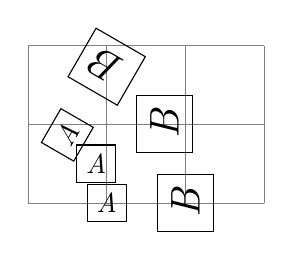
\begin{tikzpicture}
  \tikzstyle{every node}=[draw]    
  \draw[style=help lines] (0,0) grid (3,2);
  \draw            (1,0) node{A}
                   (2,0) node[rotate=90,scale=1.5] {B};
  \draw[rotate=30] (1,0) node{A}
                   (2,0) node[rotate=90,scale=1.5] {B};
  \draw[rotate=60] (1,0) node[transform shape] {A}
                   (2,0) node[transform shape,rotate=90,scale=1.5] {B};
\end{tikzpicture}
\end{codeexample}
\end{enumerate}



\subsection{Placing Nodes on a Line or Curve}

Until now, we always placed node on a coordinate that is mentioned in
the path. Often, however, we wish to place nodes on ``the middle'' of
a line and we do not wish to compute these coordinates ``by hand.''
To facilitate such placements, \tikzname\ allows you to specify that a
certain node should be somewhere ``on'' a line. There are two ways of
specifying this: Either explicitly by using the |pos| option or
implicitly by placing the node ``inside'' a path operation. These two
ways are described in the following.



\subsubsection{Explicit Use of the Position Option}

\label{section-pos-option}

\begin{itemize}
  \itemoption{pos}|=|\meta{fraction}
  When this option is given, the node is not anchored on the last
  coordinate. Rather, it is anchored on some point on the line from
  the previous coordinate to the current point. The \meta{fraction}
  dictates how ``far'' on the line the point should be. A
  \meta{fraction} or 0 is the previous coordinate, 1 is the current
  one, everything else is in between. In particular, 0.5 is the
  middle.  

  Now, what is ``the previous line''? This depends on the previous
  path construction operation.

  In the simplest case, the previous path operation was a ``line-to''
  operation, that is, a  |--|\meta{coordinate} operation:
\begin{codeexample}[]
\tikz \draw (0,0) -- (3,1)
    node[pos=0]{0} node[pos=0.5]{1/2} node[pos=0.9]{9/10};
\end{codeexample}

  The next case is the curve-to operation (the |..| operation). In this
  case, the ``middle'' of the curve, that is, the position |0.5| is
  not necessarily the point at the exact half distance on the
  line. Rather, it is some point at ``time'' 0.5 of a point traveling
  from the start of the curve, where it is at time 0, to the end of
  the curve, which it reaches at time 0.5. The ``speed'' of the point
  depends on the length of the support vectors (the vectors that
  connect the start and end points to the control points). The exact
  math is a bit complicated (depending on your point of view, of
  course); you may wish to consult a good book on computer graphics
  and B�zier curves if you are intrigued. 
\begin{codeexample}[]
  \tikz \draw (0,0) .. controls +(right:3.5cm) and +(right:3.5cm) .. (0,3)
    \foreach \p in {0,0.125,...,1} {node[pos=\p]{\p}};
\end{codeexample}

  Another interesting case are the horizontal/vertical line-to operations
  \verb!|-! and \verb!-|!. For them, the position (or time) |0.5| is
  exactly the corner point.

\begin{codeexample}[]
\tikz \draw (0,0) |- (3,1)
  node[pos=0]{0} node[pos=0.5]{1/2} node[pos=0.9]{9/10};
\end{codeexample}

\begin{codeexample}[]
\tikz \draw (0,0) -| (3,1)
  node[pos=0]{0} node[pos=0.5]{1/2} node[pos=0.9]{9/10};
\end{codeexample}

  For all other path construction operations, \emph{the position
  placement does not work}, currently. This will hopefully change in
  the future (especially for the arc operation).  
  \itemoption{sloped}
  This option causes the node to be rotated such that a horizontal
  line becomes a tangent to the curve. The rotation will always be
  done in such a way that text is never ``upside down.'' If you really
  need upside down text, use |[rotate=180]|.
\begin{codeexample}[]
\tikz \draw (0,0) .. controls +(up:2cm) and +(left:2cm) .. (1,3)
    \foreach \p in {0,0.25,...,1} {node[sloped,above,pos=\p]{\p}};
\end{codeexample}
\begin{codeexample}[]
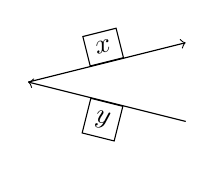
\begin{tikzpicture}[->]
  \draw (0,0)   -- (2,0.5) node[midway,sloped,above] {$x$};
  \draw (2,-.5) -- (0,0)   node[midway,sloped,below] {$y$};
\end{tikzpicture}
\end{codeexample}
\end{itemize}


There exist styles for specifying positions a bit less ``technically'':
\begin{itemize}
  \itemstyle{midway}
  is set to |pos=0.5|.
\begin{codeexample}[]
\tikz \draw (0,0) .. controls +(up:2cm) and +(left:3cm) .. (1,5)
       node[at end]          {|at end|}
       node[very near end]   {|very near end|}
       node[near end]        {|near end|}
       node[midway]          {|midway|}
       node[near start]      {|near start|}
       node[very near start] {|very near start|}
       node[at start]        {|at start|};
\end{codeexample}
  \itemstyle{near start}
  is set to |pos=0.25|.
  \itemstyle{near end}
  is set to |pos=0.75|.
  \itemstyle{very near start}
  is set to |pos=0.125|.
  \itemstyle{very near end}
  is set to |pos=0.875|.
  \itemstyle{at start}
  is set to |pos=0|.
  \itemstyle{at end}
  is set to |pos=1|.
\end{itemize}


\subsubsection{Implicit Use of the Position Option}

When you wish to place a node on the line |(0,0) -- (1,1)|,
it is natural to specify the node not following the |(1,1)|, but
``somewhere in the middle.'' This is, indeed, possible and you can
write |(0,0) -- node{a} (1,1)| to place a node midway between |(0,0)| and
|(1,1)|.

What happens is the following: The syntax of the line-to path
operation is actually |--|
\opt{|node|\meta{node specification}}\meta{coordinate}. (It is even
possible to give multiple nodes in this way.) When the optional
|node| is encountered, that is, 
when the |--| is directly followed by |node|, then the
specification(s) are read and ``stored away.'' Then, after the
\meta{coordinate} has finally been reached, they are inserted again,
but with the |pos| option set.

There are two things to note about this: When a node specification is
``stored,'' its catcodes become fixed. This means that you cannot use
overly complicated verbatim text in them. If you really need, say, a
verbatim text, you will have to put it in a normal node following the
coordinate and add the |pos| option.

Second, which |pos| is chosen for the node? The position is inherited
from the surrounding scope. However, this holds only for nodes
specified in this implicit way. Thus, if you add the option
|[near end]| to a scope, this does not mean that \emph{all} nodes given
in this scope will be put on near the end of lines. Only the nodes
for which an implicit |pos| is added will be placed near the
end. Typically, this is what you want. Here are some examples that
should make this clearer:

\begin{codeexample}[]
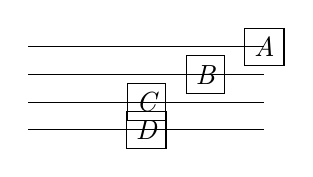
\begin{tikzpicture}[near end]
  \draw (0cm,4em) -- (3cm,4em) node{A};    
  \draw (0cm,3em) --           node{B}          (3cm,3em);
  \draw (0cm,2em) --           node[midway] {C} (3cm,2em);
  \draw (0cm,1em) -- (3cm,1em) node[midway] {D} ;
\end{tikzpicture}
\end{codeexample}

Like the line-to operation, the curve-to operation |..| also allows you to
specify nodes ``inside'' the operation. After both the first |..| and
also after the second |..| you can place node specifications. Like for
the |--| operation, these will be collected and then reinserted after
the operation with the |pos| option set.


\subsection{Connecting Nodes}

Once you have defined a node and given it a name, you can use this
name to reference it. This can be done in two ways, see also
Section~\ref{section-node-coordinates}. Suppose you have said
|\path(0,0) node(x) {Hello World!};| in order to define a node named |x|. 
\begin{enumerate}
\item
  Once the node |x| has been defined, you can use
  |(x.|\meta{anchor}|)| wherever you would normally use a normal
  coordinate. This will yield the position at which the given
  \meta{anchor} is in the picture. Note that transformations do not
  apply to this coordinate, that is, |(x.north)| will be the northern
  anchor of |x| even if you have said |scale=3| or |xshift=4cm|. This
  is usually what you would expect.
\item
  You can also just use |(x)| as a coordinate. In most cases, this
  gives the same coordinate as |(x.center)|. Indeed, if the |shape| of
  |x| is |coordinate|, then |(x)| and |(x.center)| have exactly the
  same effect.

  However, for most other shapes, some path construction operations like
  |--| try to be ``clever'' when this they are asked to draw a line
  from such a coordinate or to such a coordinate. When you say
  |(x)--(1,1)|, the |--| path operation will not draw a line from the center
  of |x|, but \emph{from the border} of |x| in the direction going
  towards |(1,1)|. Likewise, |(1,1)--(x)| will also have the line
  end on the border in the direction coming from |(1,1)|.

  In addition to |--|, the curve-to path operation |..| and the path
  operations \verb!-|! and \verb!|-! will also handle nodes without
  anchors correctly. Here is an example, see also
  Section~\ref{section-node-coordinates}:
\begin{codeexample}[]
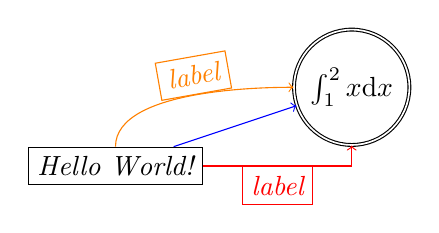
\begin{tikzpicture}
  \path (0,0) node             (x) {Hello World!}
        (3,1) node[circle,draw](y) {$\int_1^2 x \mathrm d x$};

  \draw[->,blue]   (x) -- (y);
  \draw[->,red]    (x) -| node[near start,below] {label} (y);
  \draw[->,orange] (x) .. controls +(up:1cm) and +(left:1cm) .. node[above,sloped] {label} (y);
\end{tikzpicture}
\end{codeexample}
\end{enumerate}





\subsection{Predefined Shapes}
\label{section-the-shapes}

\pgfname\ and \tikzname\ define three shapes, by default:
\begin{itemize}
\item
  |rectangle|,
\item
  |circle|, and
\item
  |coordinate|.
\end{itemize}
By loading library packages, you can define more shapes. Currently,
the package |pgflibraryshapes| defines
\begin{itemize}
\item
  |ellipse|.
\end{itemize}

The exact behaviour of these shapes differs, shapes defined for more
special purposes (like a, say, transistor shape) will have even more
custom behaviors. However, there are some options that apply to most
shapes:
\begin{itemize}
  \itemoption{inner sep}|=|\meta{dimension}
  An additional (invisible) separation space of \meta{dimension} will
  be added inside the shape, between the text and the shape's
  background path. The effect is as if you had added appropriate
  horizontal and vertical skips at the beginning and end of the text
  to make it a bit ``larger.'' The default |inner sep| is the size of
  a normal space. 

\begin{codeexample}[]
\begin{tikzpicture}
  \draw (0,0)     node[inner sep=0pt,draw] {tight}
        (0cm,2em) node[inner sep=5pt,draw] {loose}
        (0cm,4em) node[fill=examplefill]   {default};
\end{tikzpicture}
\end{codeexample}
  \itemoption{inner xsep}|=|\meta{dimension}
  Specifies the inner separation in the $x$-direction, only.
  \itemoption{inner ysep}|=|\meta{dimension}
  Specifies the inner separation in the $y$-direction, only.
  
  \itemoption{outer sep}|=|\meta{dimension}
  This option adds an additional (invisible) separation space of
  \meta{dimension} outside the background path. The main effect of
  this option is that all anchors will move a little ``to the
  outside.'' 

  The default for this option is half the line width. When the default
  is used and when the background path is draw, the anchors will lie
  exactly on the ``outside border'' of the path (not on the path
  itself). When the shape is filled, but not drawn, this may not be
  desirable. In this case, the |outer sep| should be set to zero
  point. 
\begin{codeexample}[]
\begin{tikzpicture}
  \draw[line width=5pt]
    (0,0) node[outer sep=0pt,fill=examplefill]     (f) {filled}
    (2,0) node[inner sep=.5\pgflinewidth+2pt,draw] (d) {drawn};

  \draw[->] (1,-1) -- (f);
  \draw[->] (1,-1) -- (d);  
\end{tikzpicture}
\end{codeexample}
  \itemoption{outer xsep}|=|\meta{dimension}
  Specifies the outer separation in the $x$-direction, only.
  \itemoption{outer ysep}|=|\meta{dimension}
  Specifies the outer separation in the $y$-direction, only.

  \itemoption{minimum height}|=|\meta{dimension}
  This option ensures that the height of the shape (including the
  inner, but ignoring the outer separation) will be at least
  \meta{dimension}. Thus, if the text plus the inner separation is not
  at least as large as \meta{dimension}, the shape will be enlarged 
  appropriately. However, if the text is already larger than
  \meta{dimension}, the shape will not be shrunk.
\begin{codeexample}[]
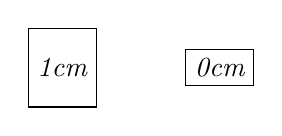
\begin{tikzpicture}
  \draw (0,0) node[minimum height=1cm,draw] {1cm}
        (2,0) node[minimum height=0cm,draw] {0cm};
\end{tikzpicture}
\end{codeexample}

  \itemoption{minimum width}|=|\meta{dimension}
  same as |minimum height|, only for the width.
\begin{codeexample}[]
\begin{tikzpicture}
  \draw (0,0) node[minimum height=2cm,minimum width=3cm,draw] {$3 \times 2$};
\end{tikzpicture}
\end{codeexample}
  \itemoption{minimum size}|=|\meta{dimension}
  sets both the minimum height and width at the same time.
\begin{codeexample}[]
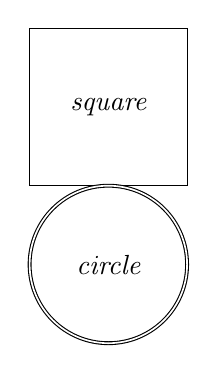
\begin{tikzpicture}
  \draw (0,0)  node[minimum size=2cm,draw] {square};
  \draw (0,-2) node[minimum size=2cm,draw,circle] {circle};
\end{tikzpicture}
\end{codeexample}
\end{itemize}

\label{section-tikz-coordinate-shape}
The |coordinate| shape is handled in a special way by \tikzname. When
a node |x| whose shape is |coordinate| is used as a coordinate |(x)|,
this has the same effect as if you had said |(x.center)|. None  of the
special ``line shortening rules'' apply in this case. This can be
useful since, normally, the line shortening causes paths to be
segmented and they cannot be used for filling. Here is an example that
demonstrates the difference: 
\begin{codeexample}[]
\begin{tikzpicture}
  \tikzstyle{every node}=[draw]
  \path[yshift=1.5cm,shape=rectangle]
    (0,0) node(a1){} (1,0) node(a2){}
    (1,1) node(a3){} (0,1) node(a4){};
  \filldraw[fill=examplefill] (a1) -- (a2) -- (a3) -- (a4);
  
  \path[shape=coordinate]
    (0,0) coordinate(b1) (1,0) coordinate(b2)
    (1,1) coordinate(b3) (0,1) coordinate(b4);
  \filldraw[fill=examplefill] (b1) -- (b2) -- (b3) -- (b4);
\end{tikzpicture}
\end{codeexample}


%%% Local Variables: 
%%% mode: latex
%%% TeX-master: "pgfmanual"
%%% End: 
